%%=============================================================================
%% Verwerking resultaten
%%=============================================================================

\chapter{Verwerking resultaten}%
\label{ch:verwerkingresultaten}

In dit hoofdstuk zullen de resultaten van de experimenten aangehaald worden. De nieuwe ontwikkelde chatbot met al zijn vereiste functionaliteiten zal ook aan bod komen. Op basis van deze gegevens en uitvoeringstijden wordt er zo tot een correct antwoord gekomen op de hoofdonderzoeksvraag in sectie \ref{sec:Hoofdonderzoeksvragen}


\section{Resultaten QR-code scanners}
\label{sec:resultatenQR-codeScanners}

In tabellen \ref{tab:3expeQR-camera}, \ref{tab:omgezette_tabel_seconds}, \ref{tab:3expeQR-scanner} en \ref{tab:omgezette_tabel2} zijn de uitvoeringstijden van de verschillende QR-code lezers waar te nemen. Als eerste schetsen we een algemeen beeld om nadien dieper in te gaan op de omgeving en de factor die de leesbaarheid en leessnelheid kan beïnvloeden. 

Hieronder vindt u per gehanteerde scan manier een overzicht van het gemiddelde, de mediaan, de standaardafwijking en de variatiecoëfficiënt van alle metingen. De meting over de beschadigde QR-codes zijn niet in acht genomen bij dit besluit. Deze komen verder aanbod.


\begin{table}[h]
    \centering
    \begin{tabular}{ |c|c|c| }
        \hline
        \multicolumn{1}{|c|}{} & \textbf{Oude QR-camera} & \textbf{Nieuwe QR-scanner} \\       
        \hline
        \textbf{\textit{Gemiddelde}} & 267,832s & 168,635s \\
        \hline
        \textbf{\textit{Mediaan}} & 217,566s & 176,180s \\
        \hline        
        \textbf{\textit{Standaardafwijking}} & 132,079s & 28,778s \\
        \hline
        \textbf{\textit{Variantiecoëfficiënt}} & 0,493 & 0,018 \\
        \hline
    \end{tabular}
    \captionsetup{justification=centering}
    \caption{De waarden in de tabel zijn uitgedrukt in seconden (s). Geven de statische gegevens terug van uitgevoerde experimenten.}
    \label{tab:nieuweScanner}
\end{table}

    
Door naar de statistische gegevens verder te kijken kunnen, we besluiten dat de nieuwe scanner beter scoort dan de oude QR-scanner op vlak van uitlezen en detecteren van een QR-code. Aangezien wij hier gewerkt hebben met totale tijdswaarden van één specifieke omgeving en één specifiek type kunnen we geen effectieve vergelijking geven tussen de verschillende factoren. We kunnen hieruit wel concluderen welke scanner er algemeen beter werkt in de geteste omgevingen en situaties.

Uit de resultaten van huidige QR-camera experiment kunnen we nog enkele conclusies nemen. Als enige tester heb ik mij zoveel mogelijk gedragen zoals een huurder de QR-code zou scannen. Wat ik vooral opmerkte bij het scannen van toegangscodes bij de huidige camera is dat de QR-code op een perfecte afstand moet gescand worden. Er kan absoluut niet afgeweken worden van de oriëntatie hoek bij het scannen. Hierdoor kunnen we concluderen dat de huurder een duidelijke indicatie moet krijgen waar en op welke afstand hij/zij de QR-code moet houden. Dit probleem was totaal niet het geval bij de nieuwe scanner opstelling. De herkenningssoftware kon nog steeds de data uitlezen ook al hield je de toegangscode in verschillende posities.

GSM vs PAPIER


Uit de experimenten met de beschadigd QR-codes kunnen we het volgende concluderen. Na het scannen van QR-code 4 (TODO verwijzing) slaagde de huidige QR-code camera er niet in om deze te detecteren. Na meerdere malen de test uit te voeren slaagde de scanner er niet in om deze uit te lezen \ref{tab:omgezette_tabel_seconds}. De gespecialiseerde QR-code scanner daarentegen kan de beschadigde QR-codes beter en sneller detecteren \ref{tab:omgezette_tabel2}. Dit bevestigt dat het herkenningsalgoritme op de USB camera minder geschikt is voor het uitlezen van beschadigde QR-codes ten opzichte van nieuwe aangekochte scanner.
    
\section{Resultaten chatbot}
\label{sec:resultatenChatbot}

\begin{figure}[h]
    \centering
    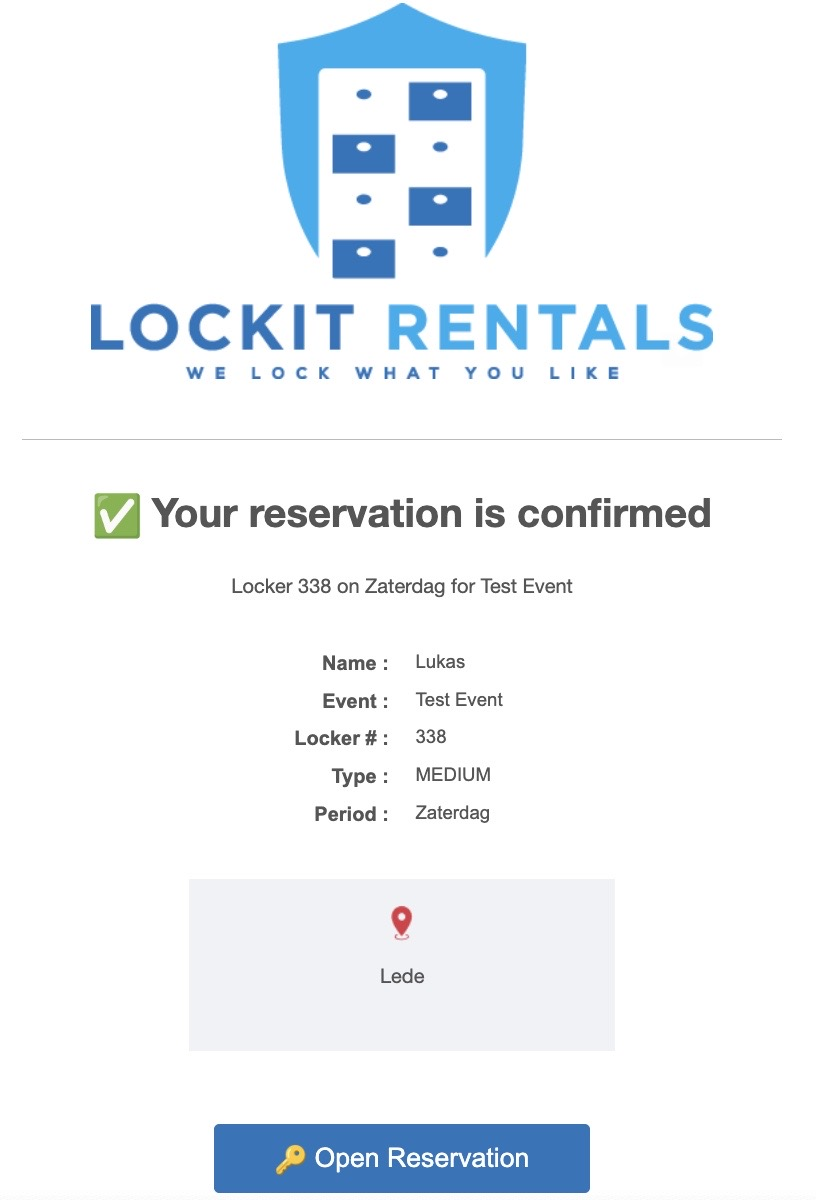
\includegraphics[width=0.5\textwidth]{graphics/F34_mailQR-code.jpg}
    \captionsetup{justification=centering, singlelinecheck=false}
    
    \caption{Een verstuurde mail afkostig van Lockit Rentals met in bijlage de teruggewonnen QR-code.}
    \label{fig:resultatEmailQR-code}
\end{figure}

\begin{figure}[h]
    \centering
    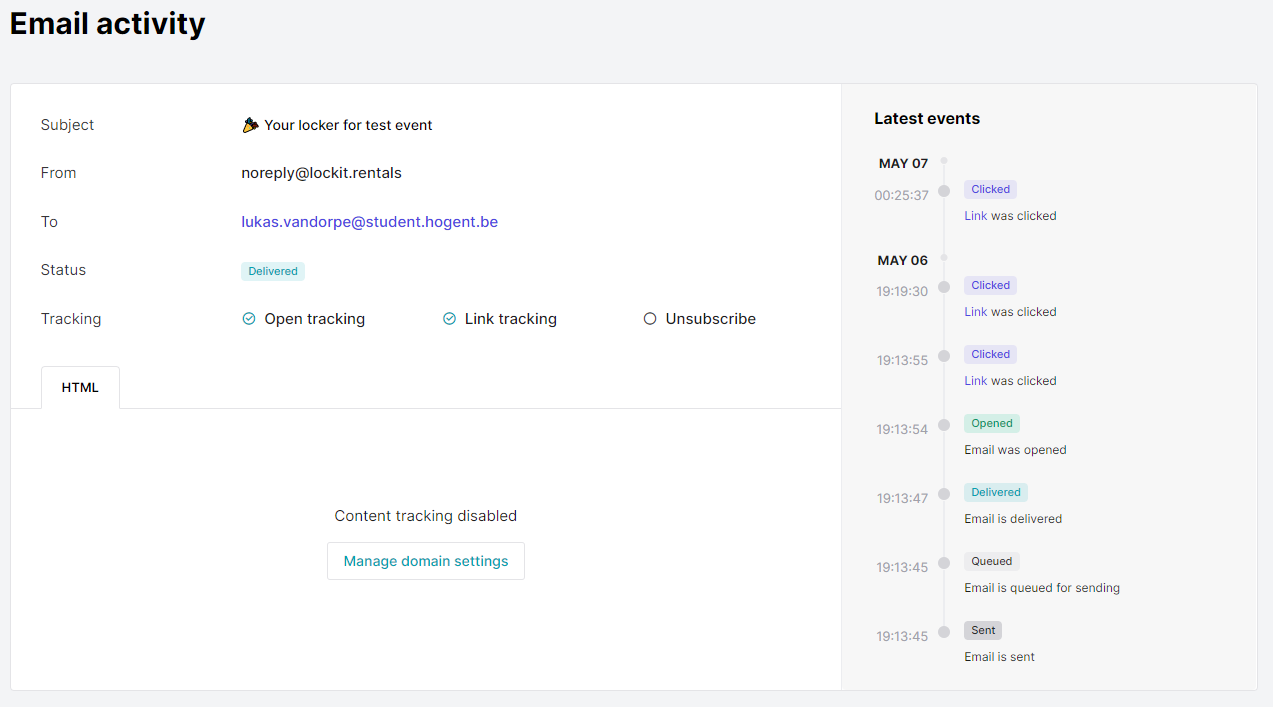
\includegraphics[width=0.8\textwidth]{graphics/F35_mailSender.png}
        \captionsetup{justification=centering,singlelinecheck=false}
    \caption{De tool 'Mail Sender' waarop we de verzonden mail kunnen traceren.}
    \label{fig:resultaatEmailSender}
\end{figure}











